\section{Landing Platform}
The team members responsible for this part of the project are Daniel Hansen, Uffe Larsen with mechanical assistance for the prototype and idea generation, and Hojat Sadat with the electronics.
\subsection{Introduction}
The function of the landing platform is to compensate for the tolerances on the CV guidance system and secure a precise landing. This is needed to establish a good connection with the battery every time. The CV guidance system should be able to make the UAV land within \SI{9}{\centi\meter} and a rotation of \SI{\pm 80}{\degree}. Thus, the dimensions of the landing pad is governed by the same numbers.

In this case the idea is to make the platform fit the IRIS drone from 3DR, although it would be preferred if the system could also be used with other UAVs or easily modified to do so.
\subsection{Idea generation}
The team came up with two general ideas for centering and alignment of the UAV, both using the IRIS' existing legs.
\subsubsection{Connector pods}
Common for both ideas is that there has to be four connector pods on the UAV. The function of these pods is to secure a stable connection of all four connections. One problem could be that the UAV will balance on three pods due to small tolerance problems. This was compensated by making the pods soft. This way they will deflect under the load of the UAV. This will ensure that all four has connection.

\begin{figure}
	\centering
	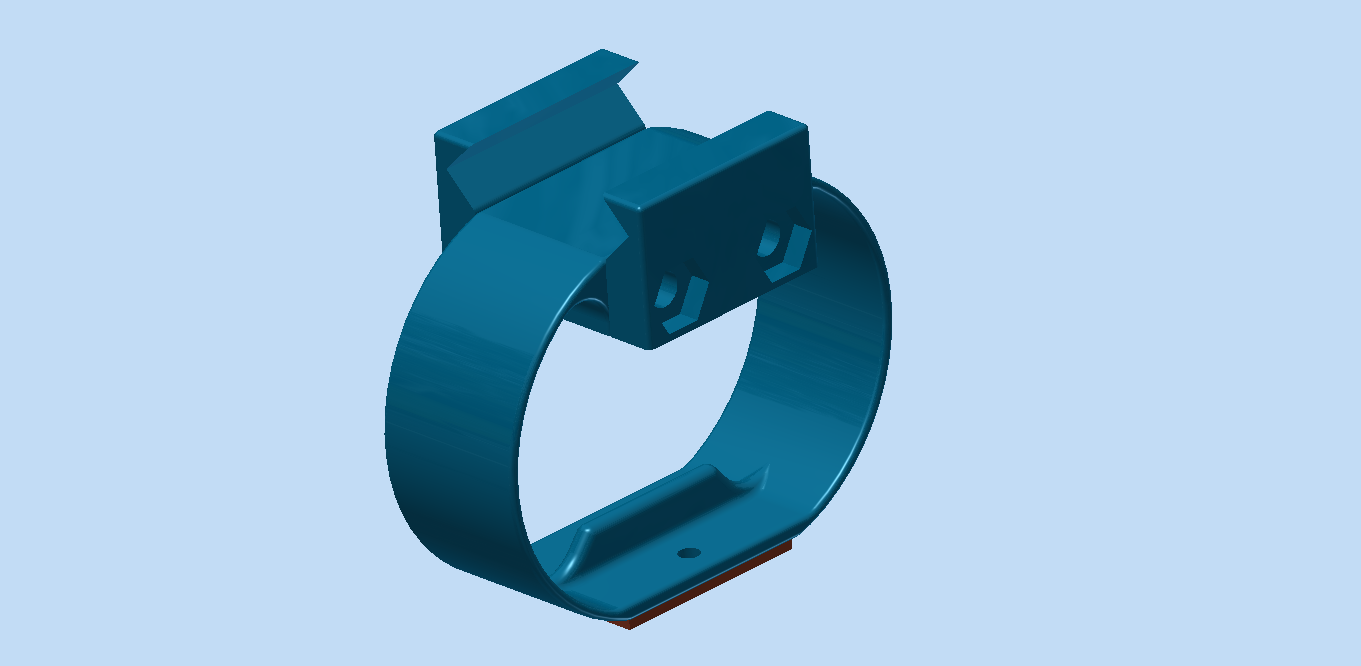
\includegraphics[width=0.8\textwidth]{imgs/connectorpod}
	\caption{CAD drawing of connector pod concept}
\end{figure}

Another challenge  was to mount them easily without modifying the drone too much, if at all. This was solved by using the mounting system under each arm on the drone to make a quick lock with two bolts.

\begin{figure}
	\centering
	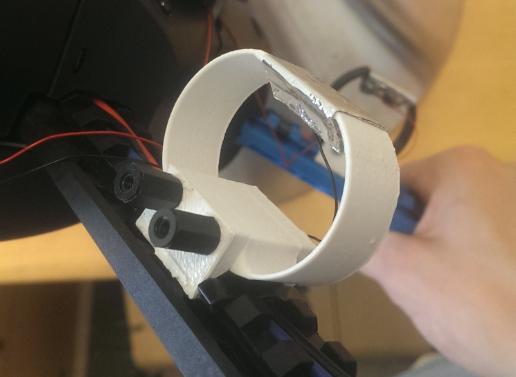
\includegraphics[width=0.8\textwidth]{imgs/connectorpod_mounted}
	\caption{Final connector pod mounted on the IRIS UAV}
	\label{fig:connectorpod_mounted}
\end{figure}

\subsubsection{Landing platform - Idea 1}
The first idea was a negative platform that would have four cone shaped holes, one for each leg. The holes will catch the legs and guide the aircraft in place. Under the body of the UAV there would be a hole in the platform to allow for a camera to see the aircraft on the sky.
\begin{figure}
	\centering
	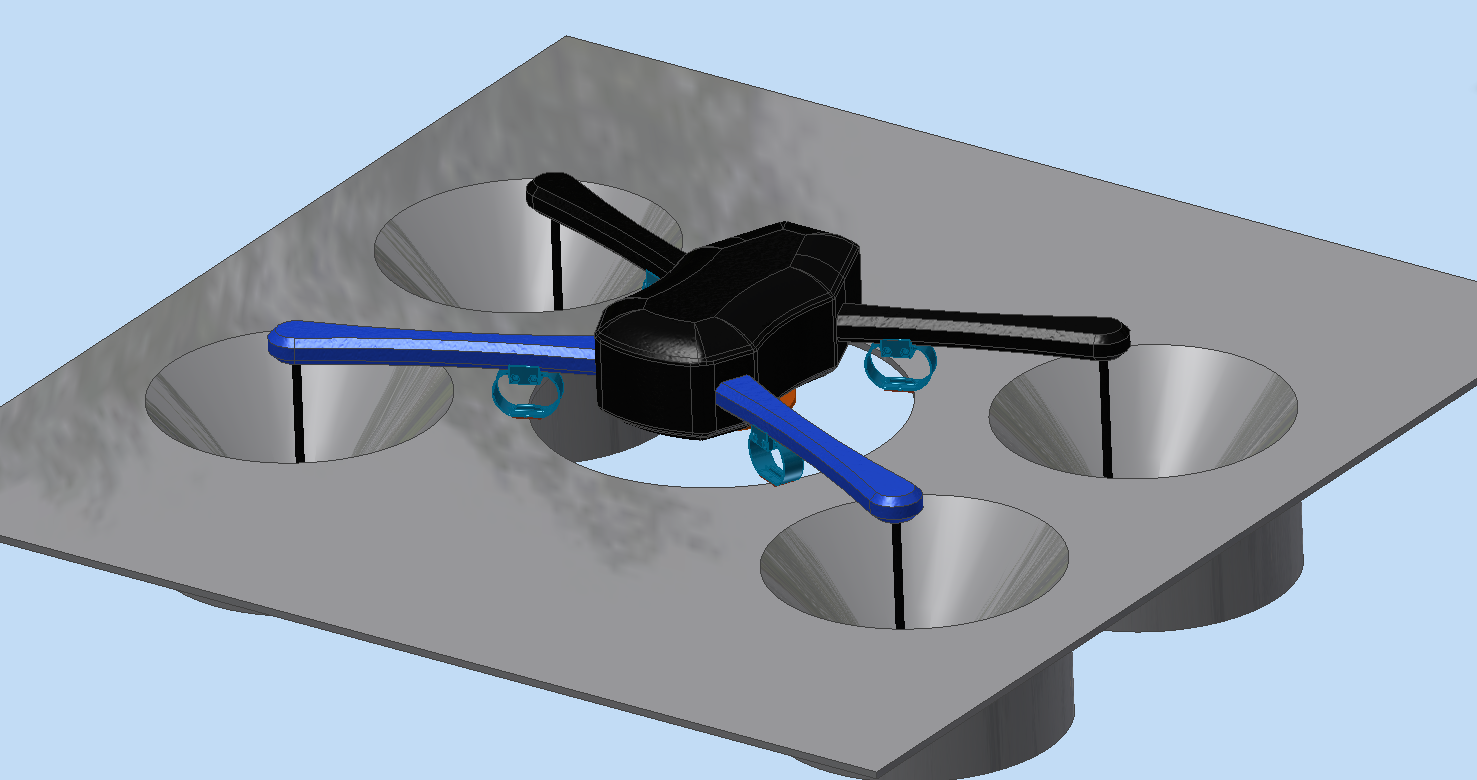
\includegraphics[width=0.8\textwidth]{imgs/mockup_idea_2}
	\caption{Idea 1 for the landing platform}
\end{figure}
\begin{center}
	\begin{tabular}{p{6.5cm} p{6.5cm}}
		\toprule
		\textbf{Advantages}                                            & Disadvantages \\\midrule
		Few parts (connectors and marker) added to the UAV.            & Ground effect on rotors. \\
		Completely locked position (x, y, z, \texttheta ) when landed. & Complicated construction. \\
			                                                           & 4 individual landing spots to hit. \\
	                                                                   & Must land rather precise as rotation plays a big role.\\\bottomrule
	\end{tabular}
\end{center}
\subsubsection{Landing platform - Idea 2}
The second idea was a positive platform, that would have one big cone with a flat top (volcano shape). On the aircraft's legs there would be mounted a ring of a flexible and light material to guide the aircraft in place. Under the body of the UAV there would be a hole in the platform to allow for a camera to see the aircraft on the sky.

\begin{figure}
	\centering
	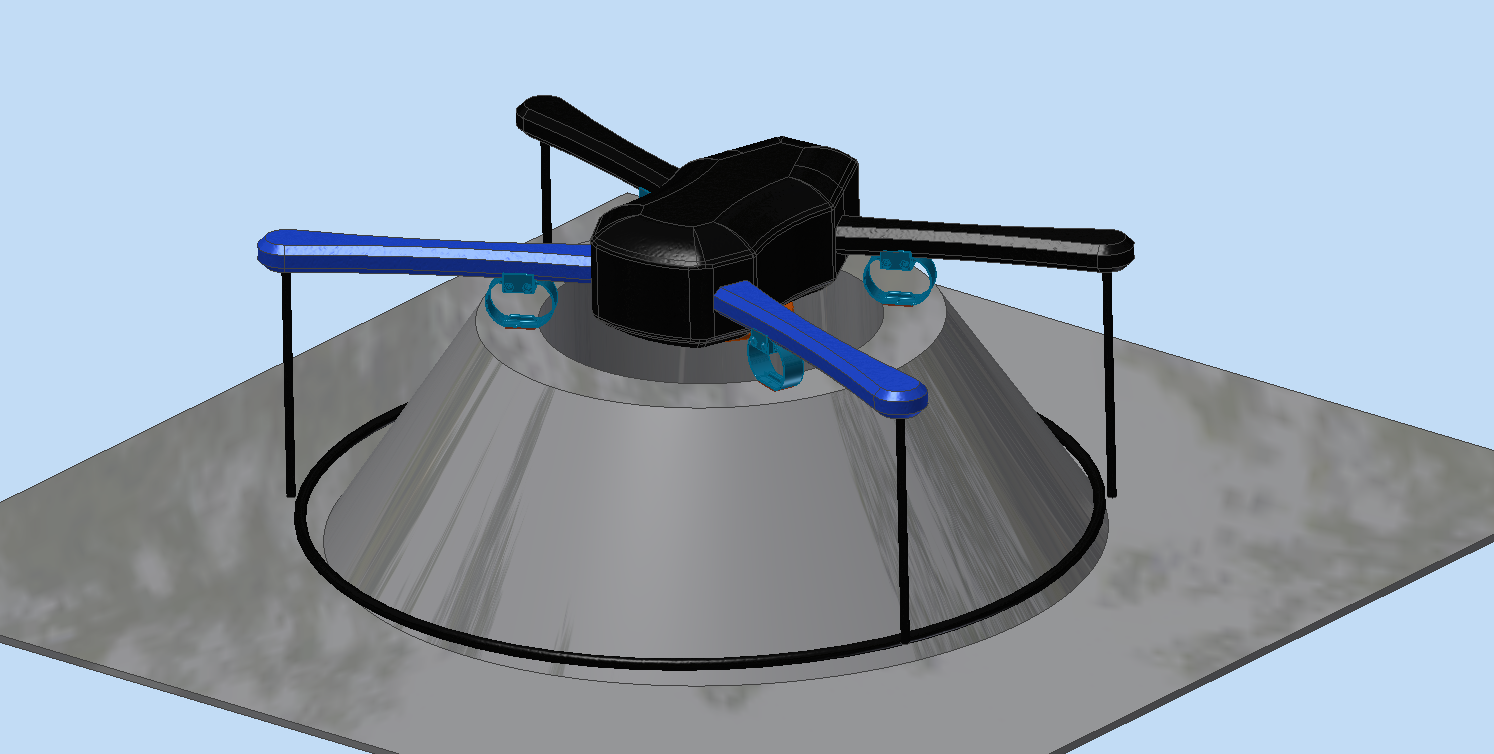
\includegraphics[width=0.8\textwidth]{imgs/mockup_idea_1}
	\caption{Idea 2 for the landing platform}
\end{figure}

\begin{center}
	\begin{tabular}{p{8cm} p{5cm}}
		\toprule
		\textbf{Advantages}                                                   & \textbf{Disadvantages} \\\midrule
		None or very little ground effect.                                    & Adds more weight to the UAV \\
		Simple construction.                                                  & \\
		One landing spot to hit with the UAV.                                 & \\
		Allows for the UAV to rotate rather much without connection problems. & \\\bottomrule
	\end{tabular}
\end{center}

As the final idea we chose idea 2. This seems to be the most tolerant idea for the CV, and it is very simple in construction compared to the little extra weight added to the UAV. Also the effect on the UAV's stability is assumed much less due to the aerodynamics of the cone compared to the flat plate on the other design which will get fairly close to the rotors (well within $5~ \times$ the rotor diameter).

\subsection{Testing of concept}
First the general concept of the idea was tested with an early prototype of the platform. This was also done to see what the smallest angle on the edges could be without tipping the drone instead of sliding it in place.

\begin{figure}
	\centering
	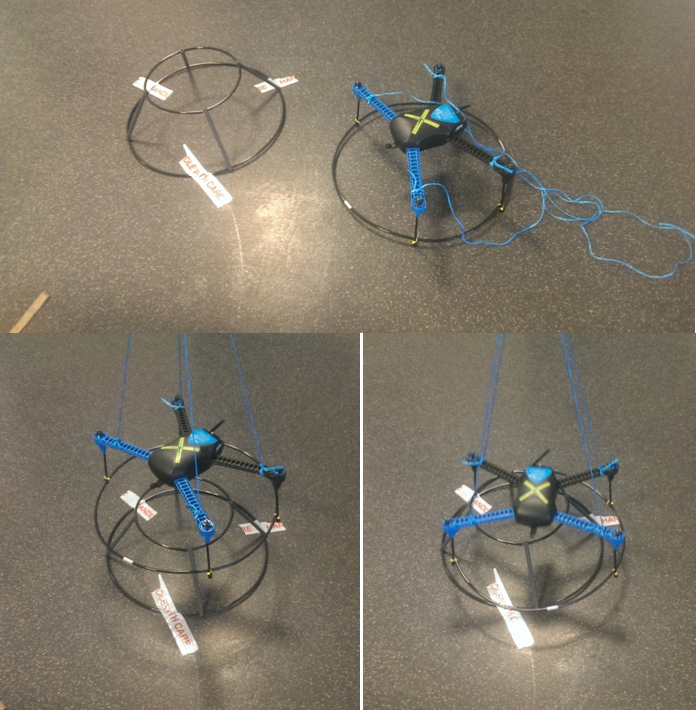
\includegraphics[width=0.8\textwidth]{imgs/prototype1_test}
	\caption{Test setup and test of the early prototype}
\end{figure}

We found that the concept works. The drone slides in place instead of tilting over. The angle should not be lower than the one the platform prototype had (\SI{55}{\degree}) at first so this was the angle we chose. If the CV gets more accurate than a radius of \SI{9}{\centi\meter} the angle can be increased and the platform will only work better.

We also made two versions of prototypes of the connector pods on a 3D printer. The first model was too stiff to bend under the weight of the UAV, so a new "weaker" model was made (see figure \vref{fig:connectorpod_mounted} and figure \vref{fig:connectorpod_crashed} - the final design can be seen in appendix \ref{sec:app3}). During flight tests we could conclude that the connectors pods are too fragile and have to be made from a different more flexible material. Figure \vref{fig:connectorpod_crashed} shows two of the connector pods after a crash.

\begin{figure}
	\centering
	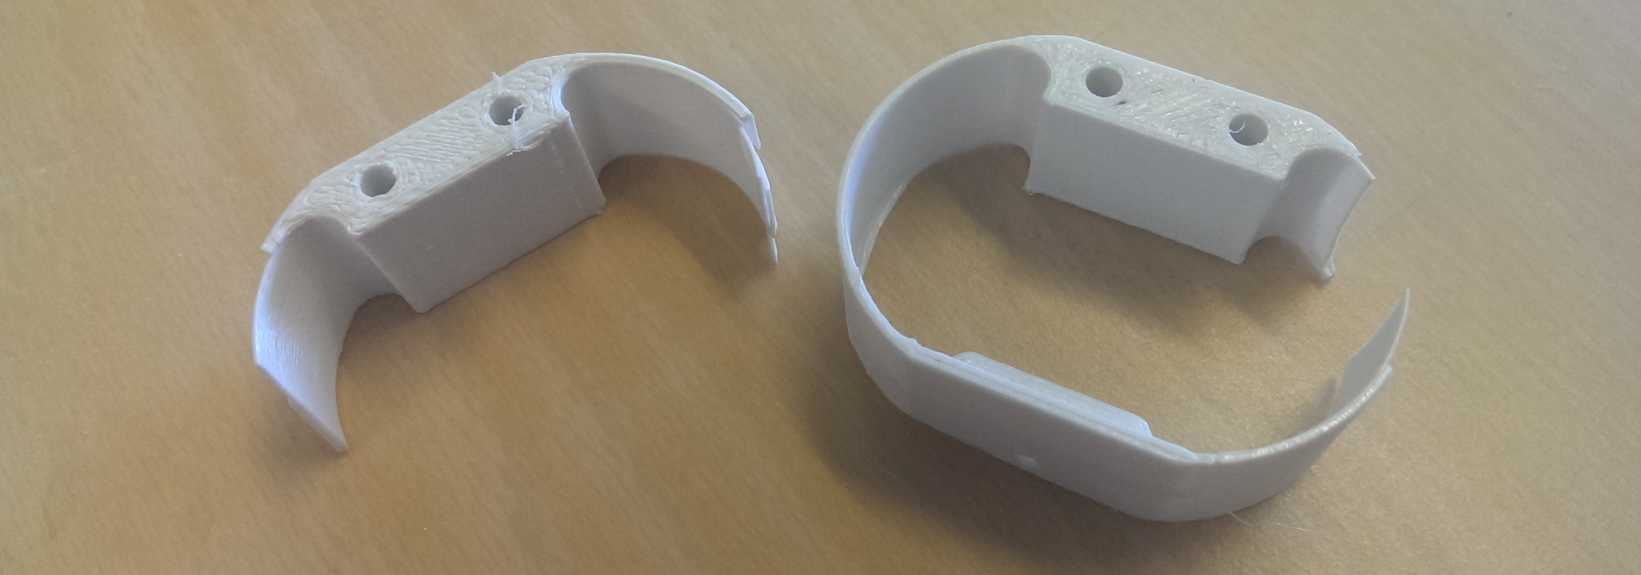
\includegraphics[width=0.8\textwidth]{imgs/connectorpod_crashed}
	\caption{Broken connector pods after a crash}
	\label{fig:connectorpod_crashed}
\end{figure}

The pods were tested to see if the connection was good. Each connector pod on the drone was connected to one of the following: ground, cell 1, cell 1-2 and cell 1-3. On the platform the four connector pads were connected to 4 LED's showing contact and the connection with each cell has been established.

As the picture above shows, the landing pad was connected to all four connector pods with success. However, the connection would be more stable if the connector pods were softer. This could be done with another plastic than the rather stiff PLA or with a softener added.

\subsection{Final design}
The final prototype was made by rolling and cutting 4 sheets of steel into the right shape and fasten them together with rivets. Then the landing pad and camera mount was cut on a laser cutter and glued together. On the landing pad four pieces of aluminum foil was used as connector pads. For engineering drawings of landing platform see appendices \ref{sec:app1} and \ref{sec:app2}.

\begin{figure}
	\centering
	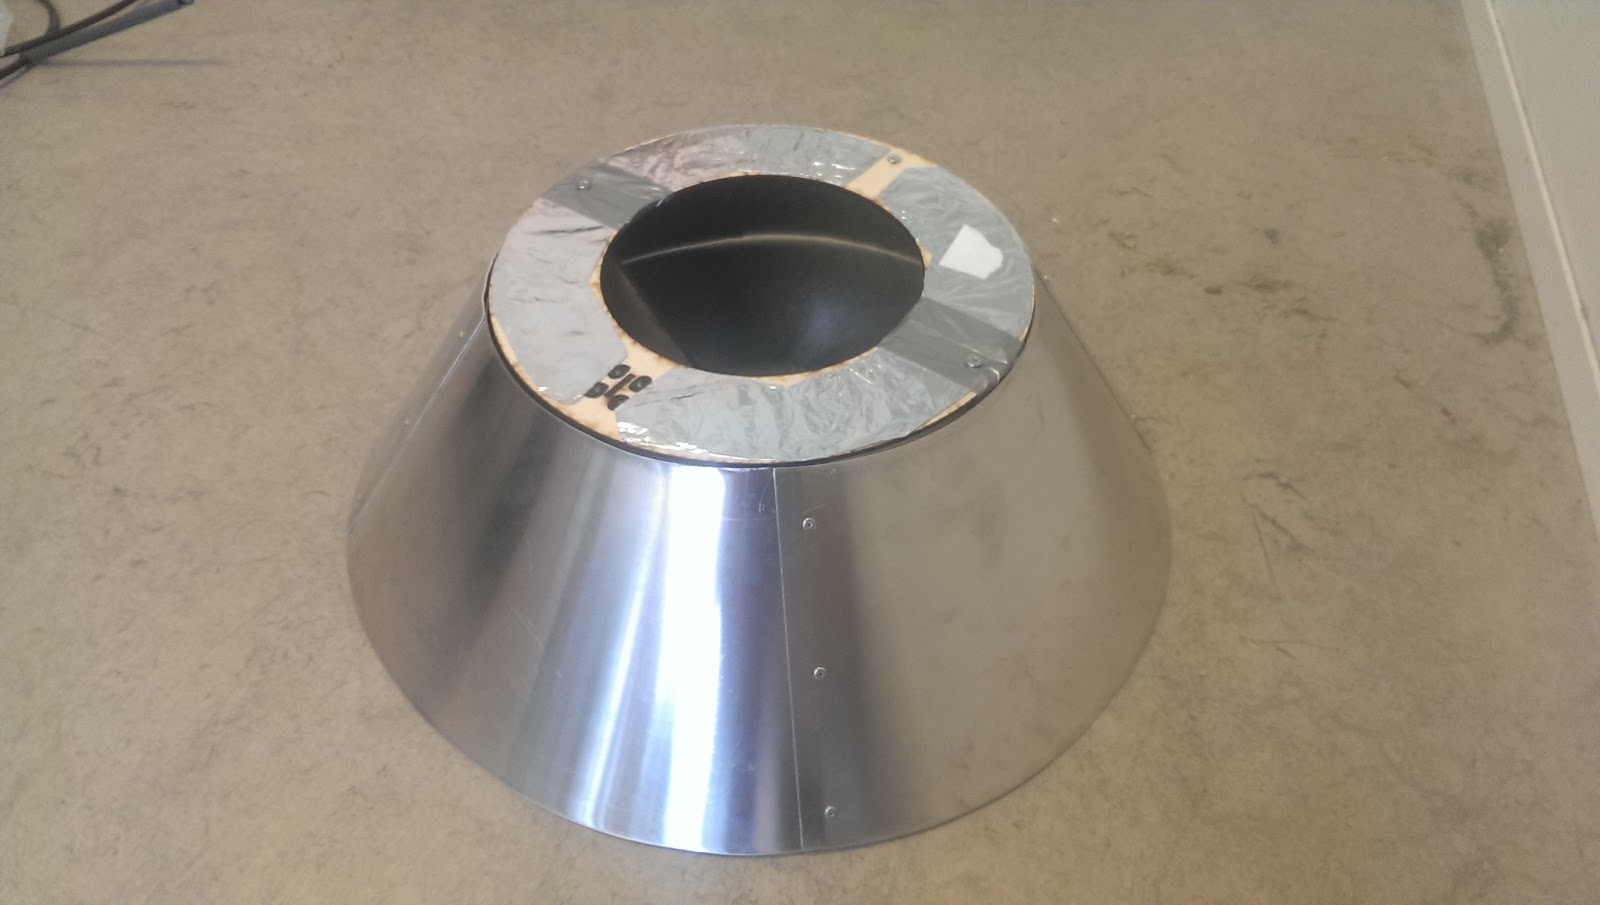
\includegraphics[width=0.8\textwidth]{imgs/cone_naked}
	\caption{Prototype of landing platform}
\end{figure}

The landing pad is mouncamerated by four “hooks” on the inside of the cone. Camera is not mounted.

\begin{figure}
	\centering
	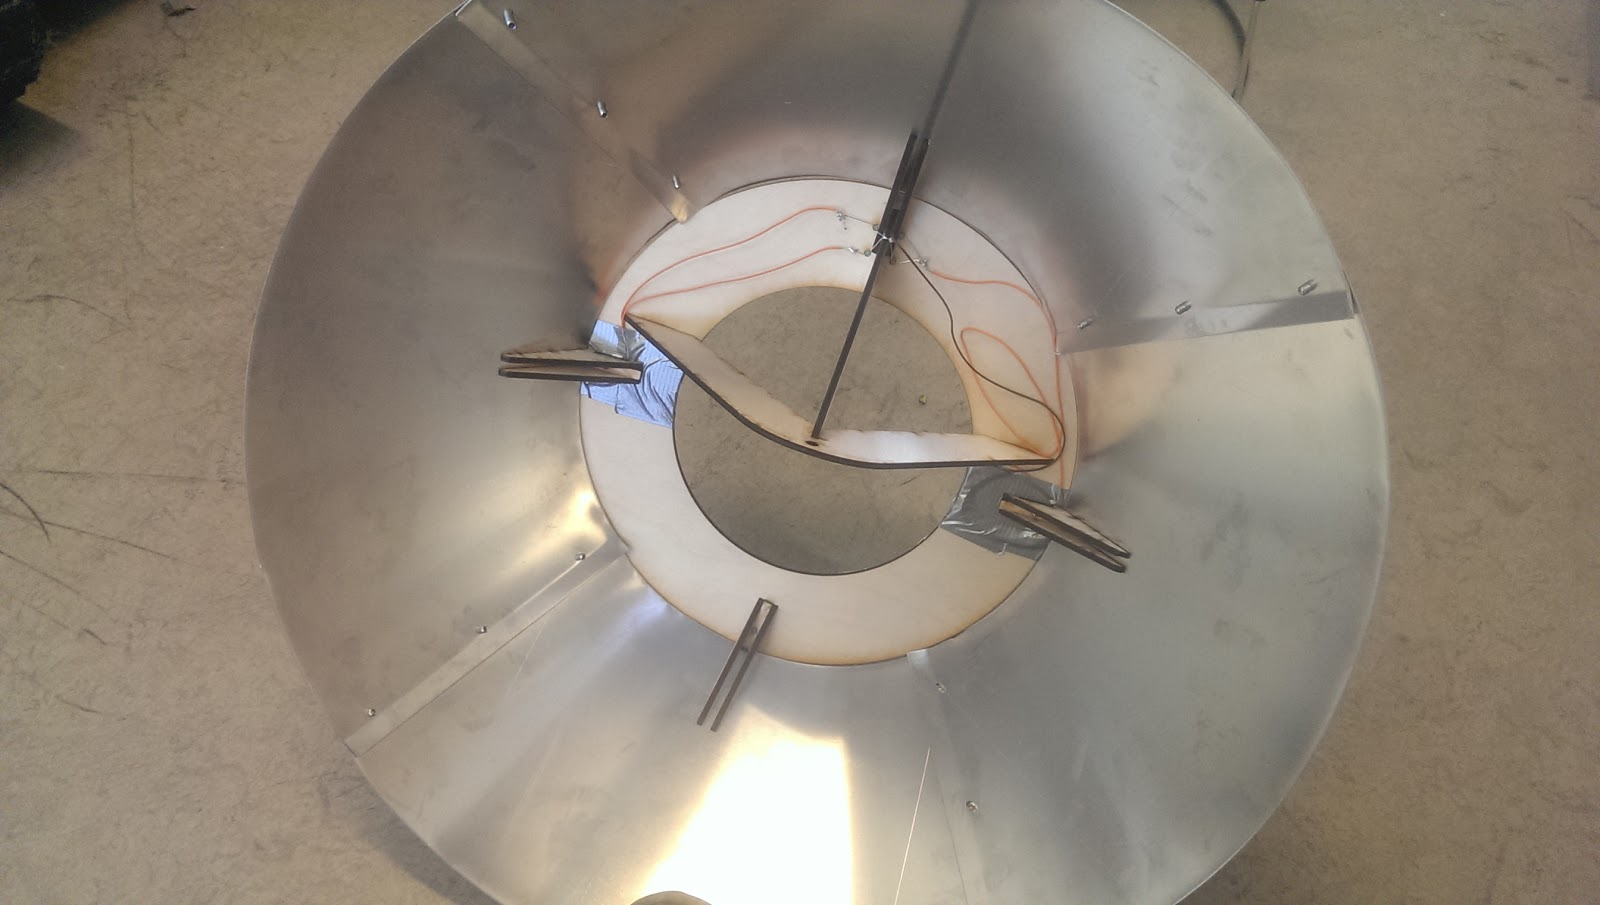
\includegraphics[width=0.8\textwidth]{imgs/cone_inside}
	\caption{Backside of the landing platform prototype}
\end{figure}

The pods were tested to see if the connection was good. Each connector pod on the UAV was connected to one of the following: ground, cell 1, cell 1-2 and cell 1-3. On the platform the four connector pads were connected to 4 LED's indicating that the connection with each cell had been established - see figure \vref{fig:prototype2_test}.

\begin{figure}
	\centering
	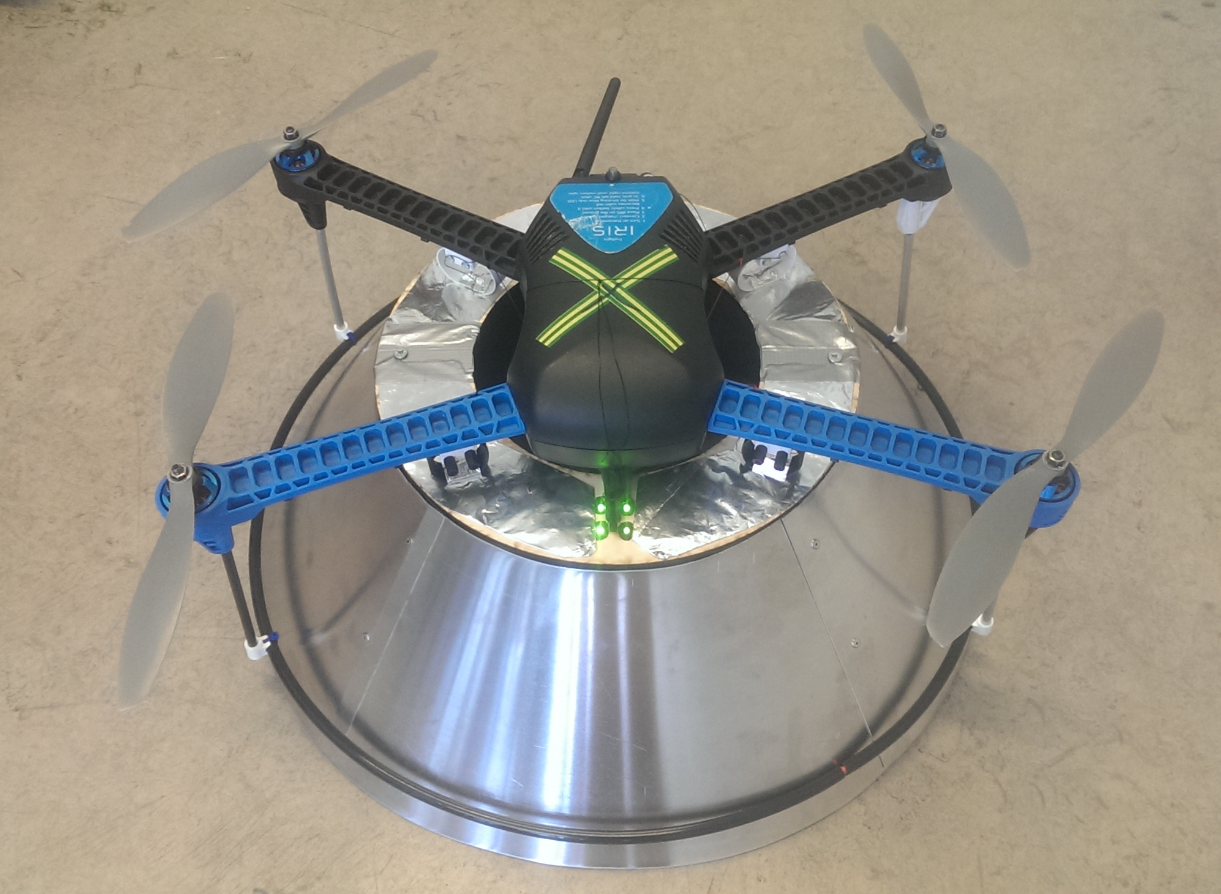
\includegraphics[width=0.8\textwidth]{imgs/prototype2_test}
	\caption{Test of docking}
	\label{fig:prototype2_test}
\end{figure}

As seen on figure \vref{fig:cone_docking_test} the front right connector pod (bottom left) is blocked with a piece of paper and the corresponding diode turns off. This is cell 1-2. Going clockwise seen from above the next pad is cell 1, ground (cuts all diodes) and cell 1-3 (this turns off the two right diodes).

\begin{figure}
	\centering
	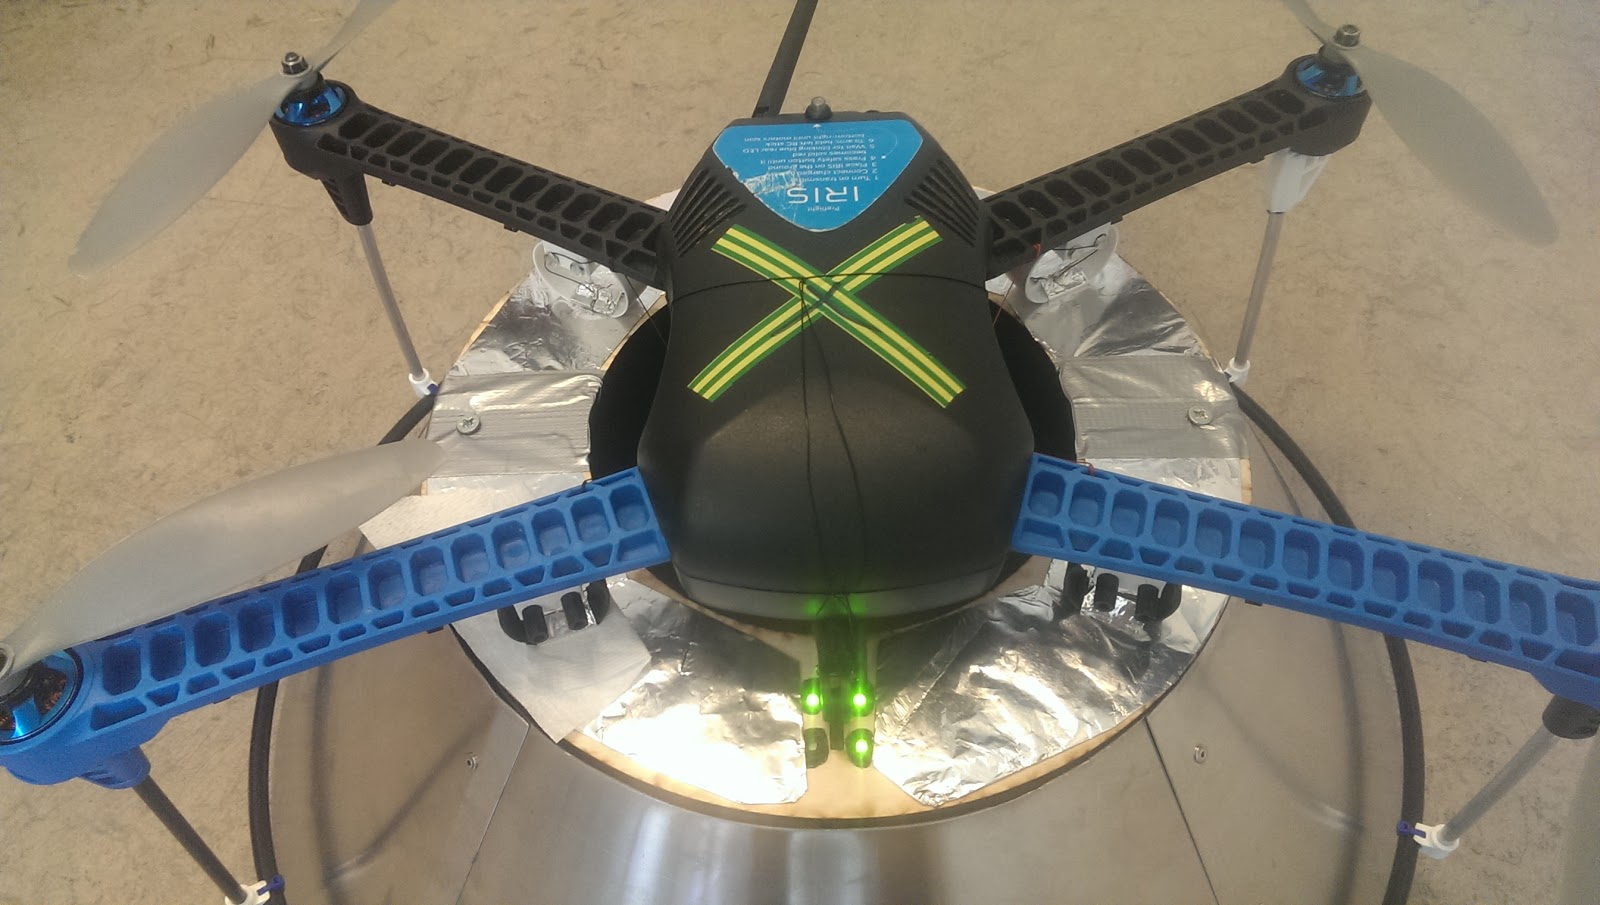
\includegraphics[width=0.8\textwidth]{imgs/cone_blocking_cell_1-2}
	\caption{Blocking cell 1-2}
	\label{fig:cone_docking_test}
\end{figure}

As the pictures above shows, through the light in the diodes, the landing pad was connected to all four connector pods with success. However the connection were unstable. It would be more stable if the connector pods were softer.

The connector pods are connected directly to the balancer plug on the UAV battery. The ground wire is connected directly. The first cell is connected without a resistor, cell 1-2 with a \SI{130}{\ohm} and finally cell 1-3 has a \SI{270}{\ohm} resistor calculated with $U=R\times I$ where $I=25$ \si{\milli\ampere} and $U$ is relatively \SI{0}{\volt}, \SI{3.4}{\volt} and \SI{6.8}{\volt}.

\begin{figure}
	\centering
	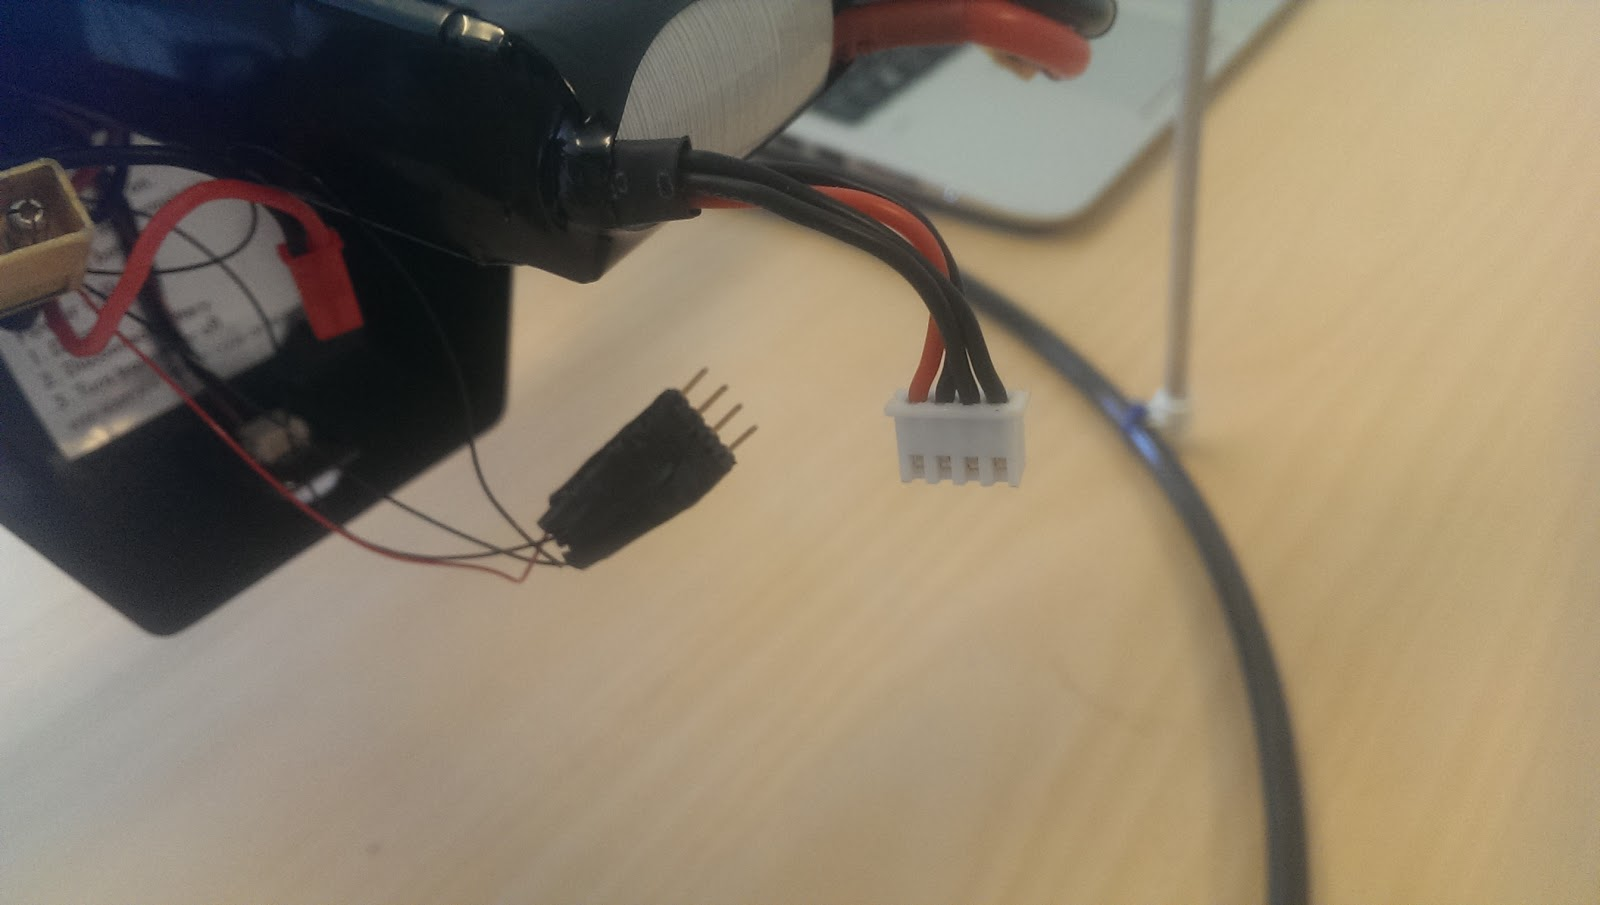
\includegraphics[width=0.8\textwidth]{imgs/battery_balancer_connector}
	\caption{Connector for connector pods}
	\label{fig:battery_balancer_connector}
\end{figure}
Figure \vref{fig:battery_balancer_connector} shows the connectors: The wires connect to, from the red wire, 1-3 cells, 1-2 cells, 1 cell and ground.

The ground base weighs \SI{944}{\g} without camera mounted. Each connector pod weighs \SI{6}{\g}. The ring weighs \SI{45}{\g}. Bolts and nuts for one connector pod weighs \SI{4}{g}. That is roughly \SI{100}{g} of weight added to the UAV with wires, resistors and connector.


\subsection{Further development}
The landing platform developed in this project has no environmental protection of the connector pads and UAV when docked. This project's main focus was to land and dock the aircraft ready to charge. For further development the concept developed in this report will have to be put in a box of some kind that will protect the UAS in bad weather.

This could be a bigger shed-like construction that will act as a windbreak to make landing easier. The shed would then have to have a roof that can open itself. Or simply just a small box that opens a lid and expose the platform in good weather and maybe even lift the landing pad free of the walls to eliminate aerodynamic problems from the box's walls

\begin{figure}
	\centering
	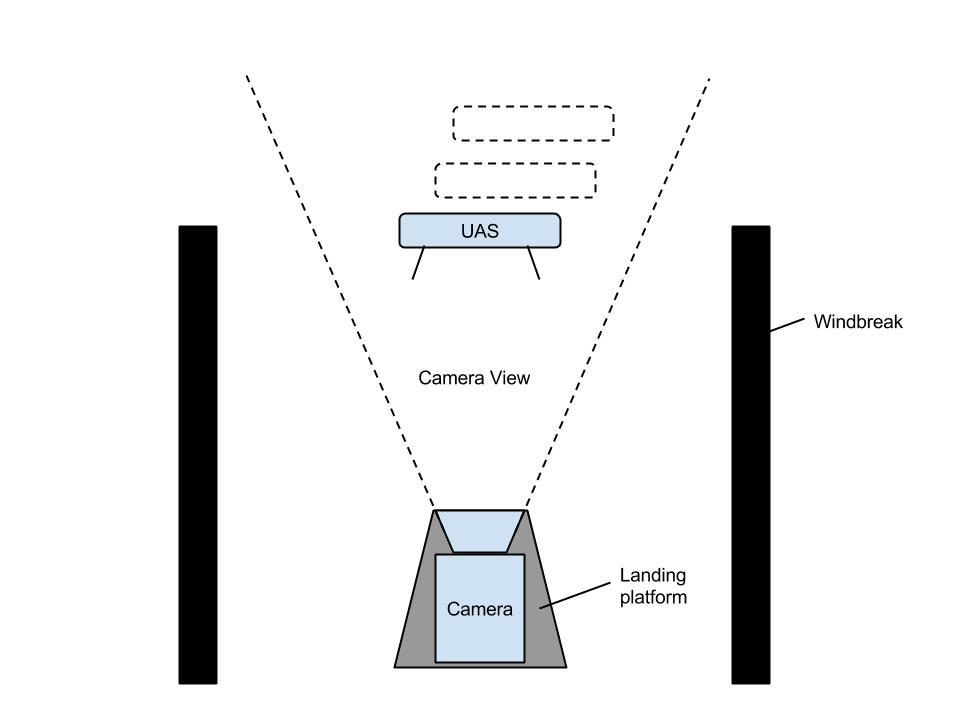
\includegraphics[width=0.8\textwidth]{imgs/landing_platform}
	\caption{General idea of landing platform}
\end{figure}

\subsection{Part conclusion}
The concept developed in this project is proven. It does the job but still need some work to be complete. If the aircraft is guided in place it docks successfully. However the prototype is indeed a prototype. The connector pods are too weak but they are also just made on a cheap 3D printer. The connector pads are made of aluminum foil which is fragile and not ideal in any way. Also the landing platform has to be protected against the environment somehow. 